\documentclass{article}

\usepackage[left=1in, right=1in, top=1in, bottom=1in]{geometry}

\usepackage{setspace}
\usepackage{fancyhdr}
\usepackage{hyperref}
\usepackage{amsthm}
\usepackage{amssymb}
\usepackage{multirow}
\usepackage{enumitem}
\usepackage{graphicx}
\usepackage{makecell}
\usepackage{booktabs}
\usepackage{titlesec}
\usepackage{amsmath}
\usepackage{pdfpages}
\usepackage{enumitem}
\usepackage{caption}


\setcounter{secnumdepth}{4}
\linespread{2.0}
\hypersetup{
    colorlinks=true,     
    urlcolor=cyan
}

\renewcommand{\qedsymbol}{\rule{0.7em}{0.7em}}

\newlength\tindent
\setlength{\tindent}{\parindent}
\setlength{\parindent}{0pt}
\renewcommand{\indent}{\hspace*{\tindent}}
\setlength{\parskip}{0em}

\newenvironment{blockquote}{%
  \par%
  \vskip1em
  \leftskip=2em\rightskip=2em%
  \noindent\ignorespaces}{%
  \par\vskip1em}

\newenvironment{blockquote2}{%
	\par%
	\vskip1em
	\leftskip=4em\rightskip=4em%
	\noindent\ignorespaces}{%
	\par\vskip1em}

\pagestyle{fancy}
\fancyhf{}
\fancyhead[LO]{STA5176}
\fancyhead[RO]{Kyle Ligon}
\fancyfoot[LO]{Final Project}
\fancyfoot[RO]{\thepage}
 
\renewcommand{\headrulewidth}{0.5pt}
\renewcommand{\footrulewidth}{0.5pt}

\begin{document}
\section*{Final Project}
\section*{Due 4-27-2018}
\subsection*{Introduction}

\indent Baltimore, Maryland, just the name of the city brings to mind countless forms of illegality and the varied levels of force spent to counteract such actions.  Whether it be the spike in recent carjackings from 2017 and the judicial systems lax consequences against the youth committing the crimes or Freddie Grey's death in the back seat of a police van after not being secured by officers after his arrest for possession of an illegal knife, Baltimore remains a city centered on the yin and yang between crimes committed and the response to those crimes.  To help people better understand the Baltimore's crime as well as add transparency to what police officers are up against, the Baltimore Police Department released crime statistics going back to December 2011.  The statistics are open for interaction in many ways including downloading as a .csv file, visualizing through plot.ly, and access through a SODA API.  In addition, this dataset was made available on kaggle.com for kernels to be produced on the data.  The goal of this project is better understand the behaviors associated with many different types of crimes in the city of Baltimore.  

\subsection*{Methods}

\indent The data was downloaded as a .csv file from \url{https://www.kaggle.com/sohier/crime-in-baltimore} and read into R for analysis.  Upon inspection, the data set contained crime and arrest records back to 12/15/2011.  The set is 276,529 rows of 15 columns including: CrimeDate, Location, Description, Inside/Outside, District, Neighborhood, and Total Incidents.  A little bit of exploratory data analysis was done to spur the questions the following hypotheses attempt to answer.  Finally, F tests were used to determine relationships of variance as well as whether variances were equal in mean tests.  T-tests were used to determine differences or equality of means after checking equality of variances.  If the equal variances requirement was violated, a Wilcoxon rank sum test was used.  In comparing percents, a two proportion z test was used to determine differences.  Finally, in looking at multiple means, an ANOVA was used to check differences with a Tukey HSD determining which pairs were significantly different.    

\begin{figure}[h]
\centering
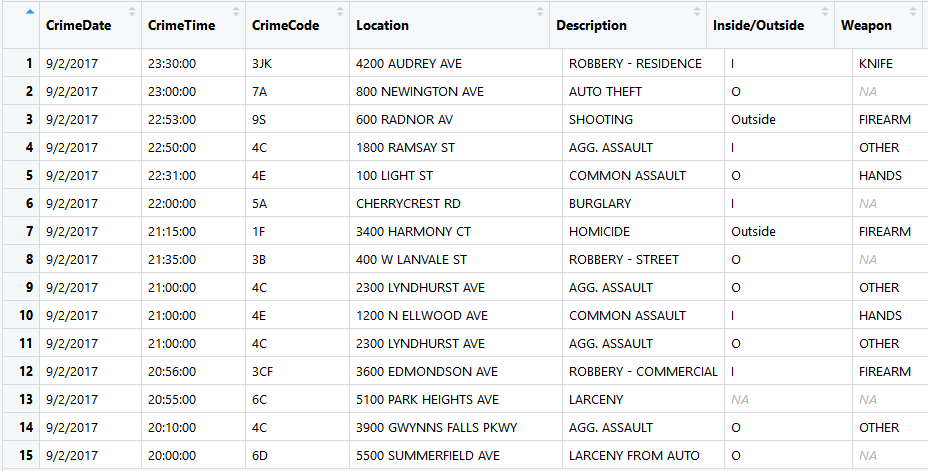
\includegraphics[width = 1.0\textwidth]{DataSetView.png}
\end{figure}


\subsection*{Hypotheses}
\indent  \textbf{Test 1:} Are the number of Arson committed in one month more varied in the Winter months (December, January, and February) in comparison to the other nine months?

$H_{0}: \sigma_{Winter}^{2} = \sigma_{SprSumWin}^{2}$ \\
$H_{1}: \sigma_{Winter}^{2} > \sigma_{SprSumWin}^{2}$ \\

\indent \textbf{Test 2:} Are there more Auto Thefts on Weekends over Weekdays?

$H_{0}: \mu_{Weekend} = \mu_{Weekday}$ \\
$H_{1}: \mu_{Weekend} > \mu_{Weekday}$ \\

\indent \textbf{Test 3:} On a given night are there more shootings inside a residence than outside?  

$H_{0}: M_{Inside} = M_{Outside}$ \\
$H_{1}: M_{Inside} < M_{Outside}$ \\

\indent \textbf{Test 4:} On any given day, if you are assaulted, is it more likely to be a common assault?  

$H_{0}: \mu_{CommonAssault} = \mu_{AggAssault}$ \\
$H_{1}: \mu_{CommonAssault} > \mu_{AggAssault}$ \\

\indent \textbf{Test 5:} Is there a district with a distinctly higher number of Burglary's in the Summer months?  If so, which are significantly different?  

$H_{0}: \mu_{Cent} = \mu_{E} = \mu_{NE} = \mu_{N} = \mu_{NW} = \mu_{SE} = \mu_{S} = \mu_{SW} = \mu_{W}$ \\
$H_{1}:$ At least one mean is different.  \\


\subsection*{Results}
\indent \textbf{Test 1:} Are the number of arson committed in one month more varied in the Winter months (December, January, and February) in comparison to the other nine months?  

\indent \indent \textbf{Data Cleaning}
\begin{blockquote}  There were 1,464 arson recorded in this data set.  When we separate them out by month, split them into Spring, Summer, and Fall (SprSumFall) and Winter divides them into a usable frame.  
\end{blockquote}

\indent \indent \textbf{Statistical Test}
\begin{blockquote}
In order to find out if the arson are more varied in a Winter month, we should use an F test to compare the variances.  Now that the two groups are divided, we calculate the sample variances and degrees of freedom for each group.  Finally, we find the F statistic(F = 0.5954) for our variance pair. 
\end{blockquote}

\newpage

\indent \textbf{Test 2:} Are there more Auto Thefts on Weekends over Weekdays?  

\indent \indent \textbf{Data Cleaning}
\begin{blockquote}
To prep the data to be worked on, we should filter down the whole table down to 28,366 robberies, carjackings, and auto thefts.  Using the \textit{wday} function from the \textbf{lubridate} package, we need a label for each day and we need to split the incidents into two data frames titled 'weekday' and 'weekend'.  Once finished, we should tally up all the events grouped on Date and looked at the distributions to make sure a test on means was appropriate.  With normal distributions in both plots, we can move on to check the variances of the two groups.  
\end{blockquote}

\indent \indent \textbf{Statistical Test(s)}
\begin{blockquote}
After checking the normal distributions, we should run an F test to on the variances to make sure they were not unequal.  I used the F test to make sure the test statistic was under the rejection region.  The F test turned up not to be statistically significant.  \\
\\
With the variances checked, I tested the means with a t-test.  When the t-test yielded a value of -1.503, I determined it wasn't statistically significant at the 95\% level.  I did not have proof that auto thefts increase on the weekends.  
\end{blockquote}

\indent \textbf{Test 3:} On a given night are there more shootings outside a residence than inside?

\indent \indent \textbf{Data Cleaning}
\begin{blockquote}
To begin, I took the data set down to just shootings after 5 PM of each day.  Upon filtering, I summed up each group of inside and outside shootings by date.  After grouping, I looked at the bar graphs to see what distribution this scenario fits.  Given the fact that they were skewed right, I chose the Wilcoxon Rank Sum test to determine if one group was shifted farther to the right than the other.     
\end{blockquote}
\indent \indent \textbf{Statistical Test}
\begin{blockquote}
After determining the test, I ran the Wilcoxon Tank Sum test on the data and arrived at a p-value of $3.6623x10^{-23}$.  Therefore, there is evidence to reject the null hypothesis that the median number of Shootings inside and outside of a building on a given night are the same.  It appears there are more shootings outside a residence at night than inside.   
\end{blockquote}
\indent \textbf{Test 4:} On a given day if you are assaulted,  is it more likely to be a common assault?

\indent \indent \textbf{Data Cleaning}
\begin{blockquote}
To arrive at probabilities of Common vs. Aggravated Assaults, I filtered the crime down to those two, summed up the total incidents of each group by day and divided them by the total number of Assaults.  Finally, I graphed the two distributions making sure the distributions were normally distributed.  
\end{blockquote}
\indent \indent \textbf{Statistical Test}
\begin{blockquote}
With normally distributed distributions, I took to evaluating if the mean of the probability of falling victim to a common assault was less than that of an aggravated assault.  I used a t-test to evaluate if that was the case.  The results came back statistically significant with a test statistic of $\chi^{2} = 8876.888$ which equates to a Z-score of $\sqrt{8876.888} = 94.217$.  The p-value associated with the test statistic is $2x10^{-16}$.  Thus, it does appear that, if one is assaulted, they are more likely to be assaulted in the form of a Common Assault as opposed to an Aggravated Assault.  
\end{blockquote}
\indent \textbf{Test 5:} Is there a District with a distinctly higher number of Burglary's in the Summer Months?  If so, which are significantly different?

\indent \indent \textbf{Data Cleaning}
\begin{blockquote}
To begin, I pulled out only the Summer months data for Burglaries, grouped by Month/Year, and summarized the total number of incidents.  There was a District equal to 'NA' that was filtered out.  After compiling all the data into a workable form, I graphed the distributions to check to see if there was a common pattern.  Seeing nothing remarkable, I went forward with an ANOVA.
\end{blockquote}
\indent \indent \textbf{Statistical Test}
\begin{blockquote}
To begin the ANOVA, I graphed the PROC MIXED results to check to see if ANOVA was appropriate.  Seeing no issues barring one outlier, I went forward to check to see if at least one mean was different than the rest.  My ANOVA came back statistically significant with an F value of 32.54.  Having validated that at least one mean was different, I proceeded with a TukeyHSD to check which pairs were different.  The following list reflects the hierarchy determined by the Statistically Significant pairwise differences: 

\begin{itemize} 
\item The Northeastern District has distinctly larger number of burglaries than all other groups.
\item The Northwestern District has a distinctly larger number of burglaries than the Western, Northern, and Eastern.
\item The Southern District has a distinctly larger number of burglaries in the Summer months over the Central, Eastern, and the Southwest.
\item The Southwest District has a distinctly larger number of burglaries in the Summer months over the Eastern, Northern, and the Western districts.  
\item The Western District has a distinctly larger number of burglaries in the Summer months over the Northern and southern Districts.
\item The Northern District has a distinctly larger number of burglaries in the Summer months over the Central and Eastern Districts.  
\item The Southeastern District has a distinctly larger number of burglaries in the Summer months over the Central and Eastern Districts.
\end{itemize}

\end{blockquote}

\subsection{Results}
\indent 
\begin{itemize}
\item In regards to arson and their variation in Winter months compared to the other three seasons, the F test statistic is lower than the rejection region, we did not have sufficient evidence to reject the hypothesis that the count of arson in the Winter months are different for the other three seasons.  It does not appear to show a difference in variation.

\item 

\item   
\end{itemize}
 

\subsection*{Conclusion}
\indent With so much data within this data set, this analysis hardly counts as a tip of the iceberg in identifying relationships between Crime(s) in Baltimore.  Going forward, more exhaustive analysis should be performed to identify actionable trends over time that the city could remedy or capitalize on to increase quality of life for its citizens.  Additionally, building a mathematical model that \textit{explains} crime numbers in the different neighborhoods could aid the city of Baltimore.  All in all, Baltimore Police Department keeping transparency at the forefront empowers citizens in and out of Baltimore to help turn around crime's hold on the city's residents.  


\subsection*{References}
City of Baltimore. (2017). BPDPart1VictimBasedCrimeData [Data file].  Retrieved from \url{https://www.kaggle.com/sohier/crime-in-baltimore/data}.  

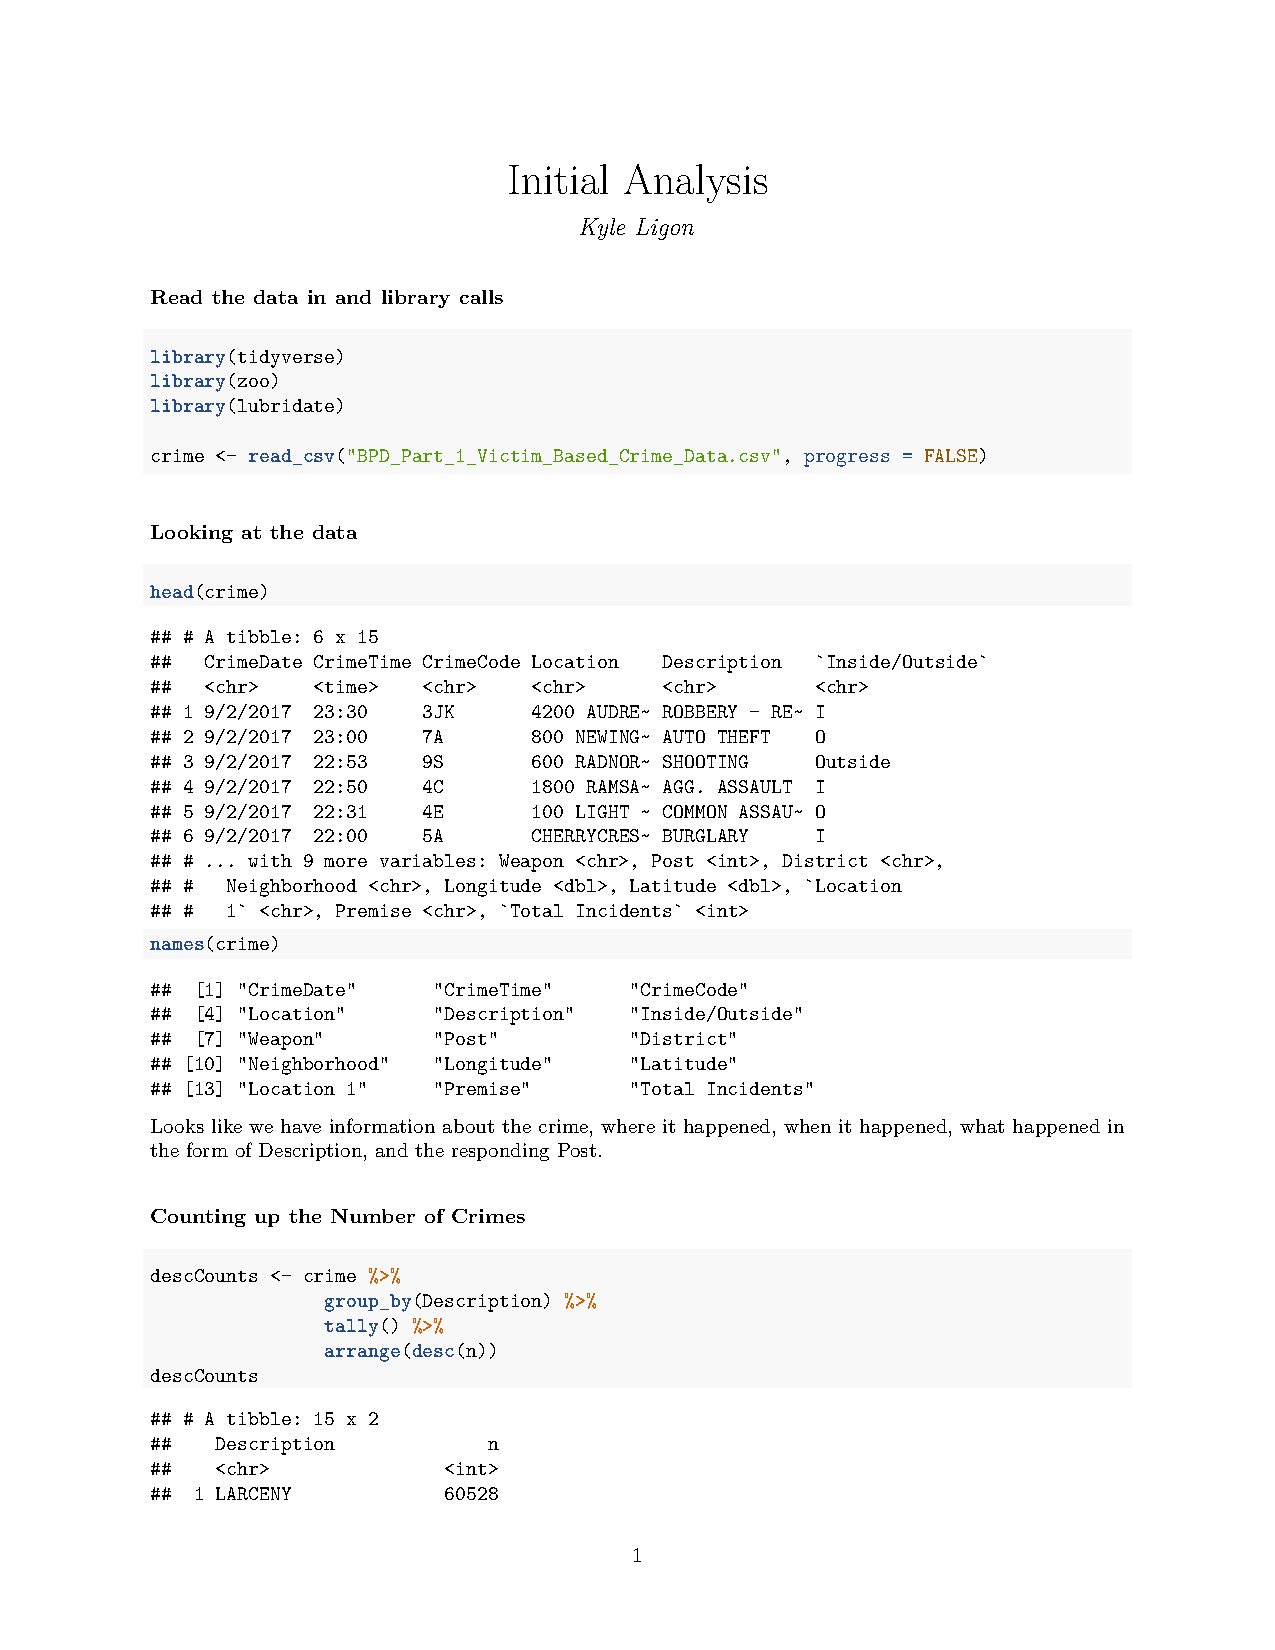
\includepdf[pages=-]{EDA_Notebook.pdf}

\end{document}